\documentclass[conference]{IEEEtran}
\usepackage{cite}
\usepackage{amsmath,amssymb,amsfonts}
\usepackage{algorithmic}
\usepackage{graphicx}
\usepackage{textcomp}
\usepackage{xcolor}

% our packages
\usepackage{todonotes}
\usepackage[caption=false]{subfig}
\usepackage{url}
\usepackage{enumitem}
\usepackage{listings}
\usepackage{boxedminipage}
\usepackage{comment}
\usepackage{multirow}
\usepackage{microtype}
\usepackage[normalem]{ulem}
\usepackage{hyperref}

%\def\BibTeX{{\rm B\kern-.05em{\sc i\kern-.025em b}\kern-.08em
%    T\kern-.1667em\lower.7ex\hbox{E}\kern-.125emX}}

% our defs
\setlist{noitemsep,leftmargin=*}
%\newenvironment{tightlist}{\begin{itemize}\setlength{\itemsep}{0pt}\setlength{\parskip}{0pt}}{\end{itemize}}
\newcommand{\mycomment}[1]{\emph{\textcolor{red}{[#1]}}}
    
\begin{document}

\title{Composable Building Blocks to Open up Processor Design}

\author{\IEEEauthorblockN{Sizhuo Zhang, Andrew Wright, Thomas Bourgeat, Arvind}
\IEEEauthorblockA{MIT CSAIL\\
\{szzhang, acwright, bthom, arvind\}@csail.mit.edu}}

\maketitle

\thispagestyle{plain}
\pagestyle{plain}

\begin{comment}
\section{Structure}
\begin{enumerate}
    \item Introduction:
    \begin{enumerate}
        \item Challenge in processor design.
        \item Structural design $\xrightarrow{}$ latency insensitive  $\xrightarrow{}$ microarchitectural races.
        \item CMD.
    \end{enumerate}
    \item Related works. (Half a column)
    \item CMD:
    \begin{enumerate}
        \item Motivating example for microarchitectural races: IQ. (Half a column).
        \item Conflict matrix: capture concurrency properties in module interfaces.
        \item CMD workflow, BSV and other HDLs, supported modular refinement.
    \end{enumerate}
    \item RiscyOO: figures (caption: we can duplicate ALU pipeline) and summary of performance numbers.
    \item Application of CMD:
    \begin{enumerate}
        \item Refine processor IP: TLB (the changes being made).
        \item Security: MI6.
        \item Validate SW-HW codesign.
    \end{enumerate}
    \item Conclusion.
    \item Acknowledgement.
\end{enumerate}
\end{comment}

\begin{abstract}
    % Maximum 149 words
    We present a framework called Composable Modular Design (CMD) to facilitate the design of out-of-order processors. In CMD, (1) The interface methods of modules provide instantaneous access and perform atomic updates to the state elements inside the module; (2) Every interface method is guarded, i.e., it cannot be applied unless it is ready; and (3) Modules are composed by atomic rules which call interface methods of different modules. A rule either successfully updates the state of all the called modules or does nothing.
    
    The atomicity properties of interfaces in CMD ensure composability when modules are refined selectively. We show the efficacy of CMD by building an out-of-order RISC-V processor which boots Linux. Modules designed using CMD (e.g., ROB, load-store unit, etc.) can be used and refined by other implementations. We believe that this framework can revolutionize architectural research and practice as the library of reusable components grows.
\end{abstract}

\section{Introduction}\label{sec:intro}
It is generally believed that modern processors are the most sophisticated hardware systems that currently exist.
Given the complexity of the design of a processor, it is split into multiple modules, which are often designed by different teams.
This partition of work leads to the following two challenges:
\begin{enumerate}
    \item Will the processor work as expected when the modules are composed together?
    \item Is it possible to do \emph{modular refinement}, i.e., refine a module without knowing the implementation details of the other modules?
\end{enumerate}
Ability to do modular refinement is necessary to meet the goal of performance/power/area (PPA), and in some sense it subsumes the functionality challenge. 

Most processors~\cite{rocketchip,boom,fabscalar,pulp} have been designed in a \emph{structural} way, i.e., modules are physical blocks connected by wires.
The implementation of one module may make implicit assumptions about the timing of input signals coming from other modules, and thus, the composed processor functions correctly if each module meets its timing assumptions and functionality.
Such timing assumptions are difficult to specify, which makes the mechanical verification of timing-assumption violations impossible.
In order to avoid rigid timing assumptions, some designers use the latency-insensitive framework, where modules communicate with each other using FIFOs.
In such frameworks a module cannot depend on the timing of other modules, and that significantly improves the flexibility in modular refinement.
Although the latency-insensitive framework has proven useful in building hardware accelerators, it is not expressive enough for processors. 
In processors, a microarchitectural event may need to access and modify the states in multiple modules \emph{atomically}. 
This is because different microarchitectural events may race with each other in accessing the states inside modules, and such ``data races'' can make the processor implementation incorrect if an event fails to perform all its accesses atomically with respect to other events.
Here we list several race cases in the out-of-order (OOO) processor we have built, and we will discuss a detailed example later in Section~\ref{sec:cmd:iq}:
\begin{enumerate}
    \item \emph{Speculation bits}:
    Often an instruction flowing through the execution pipeline carries bits to indicate the speculation events which can cause its squashing.
    There is a race in the management of these bits, because they are cleared by asynchronous events that show that the speculations were correct.
    
    \item \emph{Memory address disambiguation}:
    A load in the load queue searches the store queue for forwarding, and a store in the store queue may update its address and search the load queue for detecting memory-dependency violations. 
    There is a race if the addresses are the same.
    
    \item \emph{Partially overlapped addresses}:
    A load also searches through older stores for stalls due to partially overlapped addresses, and a store should wake up younger loads stalled by it when the store is written to the L1 cache.
    There is a race if the addresses overlaps partially.
    
    \item \emph{Distributed cache coherence protocols}:
    A race condition arises when a parent is trying to downgrade a child's entry while it is receiving the eviction of the same entry from the child.
\end{enumerate}

A non-modular solution to these race problems is to put all the interacting components in one module.
However, doing so in complex designs leads to big monolithic modules.

In this paper, we present the Composable Modular Design (CMD) framework, which permits state changes in multiple modules \emph{atomically}.
CMD uses the following two techniques to achieve composability and atomicity:
\begin{enumerate}
    \item \emph{modules with guarded interface methods}, and
    \item \emph{atomic rules} that glue modules together by calling the methods of modules.
\end{enumerate}

In CMD, a module is like an object in an object-oriented programming language, and can be manipulated only by its interface methods.
A method provides combinational access and performs atomic updates to the state elements inside the module.
In addition, every interface method is \emph{guarded}, that is, there is an implicit guard (a ready signal) on every method which must be true before the method can be invoked (enabled).
For example, the guard signal for the enqueue method of a FIFO is simply the not-full condition.
CMD subsumes the traditional latency-insensitive framework by admitting systems where each interface method of every module simply enqueues or dequeues FIFOs.

Unlike the structural designs, modules in CMD are manipulated by the special glue logic, i.e., atomic rules, which is a collection of calls to the methods of one or more modules.
An atomic rule is like an atomic transaction, which either updates the states of all the called modules  or does nothing.
Of course, a method can execute only if its guard is true; therefore, the guards of all the methods called by a rule must be true simultaneously.
In CMD, each microarchitectural event (which happens in a single cycle) is expressed as an atomic rule.
Atomicity ensures that refinement of a module will not affect how it is used by the rules, i.e., modules are much more composable.

This paper makes the following contributions:
\begin{enumerate}
    \item Composable Modular Design (CMD) flow, a new framework for implementing complex and realistic microarchitectures;
    
    \item A parameterized and modular OOO processor, \emph{RiscyOO} built using the CMD framework, which is released at \texttt{\url{https://github.com/csail-csg/riscy-OOO}} under the MIT License;
    
    \item Applications of the CMD framework and the RiscyOO processor.
\end{enumerate}

\noindent\textbf{Paper organization:}
Section~\ref{sec:related} presents related works.
Section~\ref{sec:cmd} describes the CMD framework.
Section~\ref{sec:ooo} introduces the RiscyOO processor built using CMD.
Section~\ref{sec:app} discusses further applications of CMD.
Section~\ref{sec:conclude} concludes the paper.

\section{Related Work}\label{sec:related}
There is a long history of processors that were designed in the academic setting.
Many of these attempts were focused on demonstrating new architectures; there was no expectation that other people would improve or refine an existing implementation.
Other attempts aimed at providing open-source processors and a corresponding framework for configuring the design.
For example, the Rocket chip generator~\cite{rocketchip} can generate SoCs with RISC-V cores that are parameterized by caches, branch predictors, degree of superscalarity, and ISA extensions.
Fabscalar~\cite{fabscalar} allows one to assemble a variety of superscalar designs from a set of predefined pipeline-stage blocks.
FabScalar have been successful in generating heterogeneous cores, but the predefined blocks are not intended to be modified themselves.
PULP~\cite{pulp} is a platform for designing low-power IoT SoCs, but the processor cores are not intended to be refined within the framework.

All these frameworks are structural compositions of predefined building blocks.
The goal of our CMD framework is more ambitious, in the sense that, in addition to parameterized designs, we want the users to be able to incorporate new microarchitectural ideas.
For example, replace a central instruction issue queue in an OOO design, with several instruction issue queues, one for each functional unit.
Traditionally, making such changes requires a deep knowledge of the internal functioning of the other blocks, otherwise, the processor is unlikely to function. 
We want to encapsulate enough properties in the interface of each block so that it can be composed without understanding the internal details.

\section{Composable Modular Design (CMD) Framework}\label{sec:cmd}

As mentioned in Section~\ref{sec:intro}, latency-insensitive frameworks are insufficient for processor designs because of races between microarchitectural events.
We first study an example race case which involves the instruction issue queue (IQ) in the OOO processor, and then show how CMD maintains atomicity and solves the race problem by extending module interfaces with concurrency properties.

\subsection{Race between Microarchitectural Events}\label{sec:cmd:iq}
Figure~\ref{fig:race:modules} shows the modules and microarchitectural events that participate in a race in the OOO processor.
Module IQ keeps unissued instructions and tracks whether their (physical) source registers are ready or not.
Module RDYB keeps one bit for each physical register, indicating whether the register has valid data or not.
Microarchitectural event {Rename} gets a new instruction from the decode stage, do renaming, \emph{checks} RDYB to see if the source registers of the instructions are ready, and \emph{enters} the instruction with the register-ready bits into IQ.
Microarchitectural event {RegWrite} happens at the end of execution pipeline when an instruction gets the value for its destination register.
The event \emph{sets} the corresponding bit in RDYB and \emph{wakes} up dependent instructions in IQ.
(There are other actions performed by the two events, but they are unrelated to the race case we are going to discuss.)

Both events are accessing the states in IQ and RDYB, thus forming a race.
If event Rename does not happen atomically with respect to event RegWrite, then the race can lead to deadlock in the processor.
Consider the case in Figure~\ref{fig:race:deadlock}.
Event Rename is processing instruction $I$ with physical source register $P3$, while event RegWrite is writing the same register $P3$.
It is possible that event Rename first checks RDYB and finds $P3$ not ready, then event RegWrite happens and cannot wake up instruction $I$ which is not yet in IQ, and finally event Rename enters $I$ into IQ.
In this case, $I$ will stuck in IQ forever, i.e., the processor deadlocks.

It is difficult for latency-insensitive frameworks to keep the atomicity of events and resolve this race problem.
A structural solution is to introduce bypass wires either in RDYB (to have Rename see the updated register-ready bits) or in IQ (to have RegWrite wake up instruction $I$).
However, the bypass wires break latency insensitivity and reduces composability.

\begin{figure}[!htb]
    \centering
    \subfloat[Modules and microarchitectural events involved in the race. Modules IQ and RDYB are represented by blocks, while microarchitectural events Rename and RegWrite are represented by clouds. Event Rename calls method \emph{check} of RDYB and method \emph{enter} of IQ. Event RegWrite calls method \emph{set} of RDYB and method \emph{wake} of IQ.\label{fig:race:modules}]{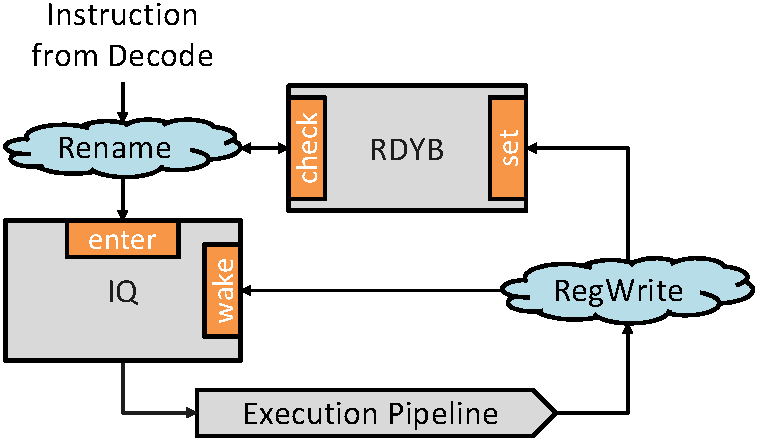
\includegraphics[width=0.8\columnwidth]{figs/race_cropped.pdf}}\\
    \subfloat[Operation sequence that leads to deadlock. Event Rename is processing instruction $I$ with source register P3 while event RegWrite is writing P3.\label{fig:race:deadlock}]{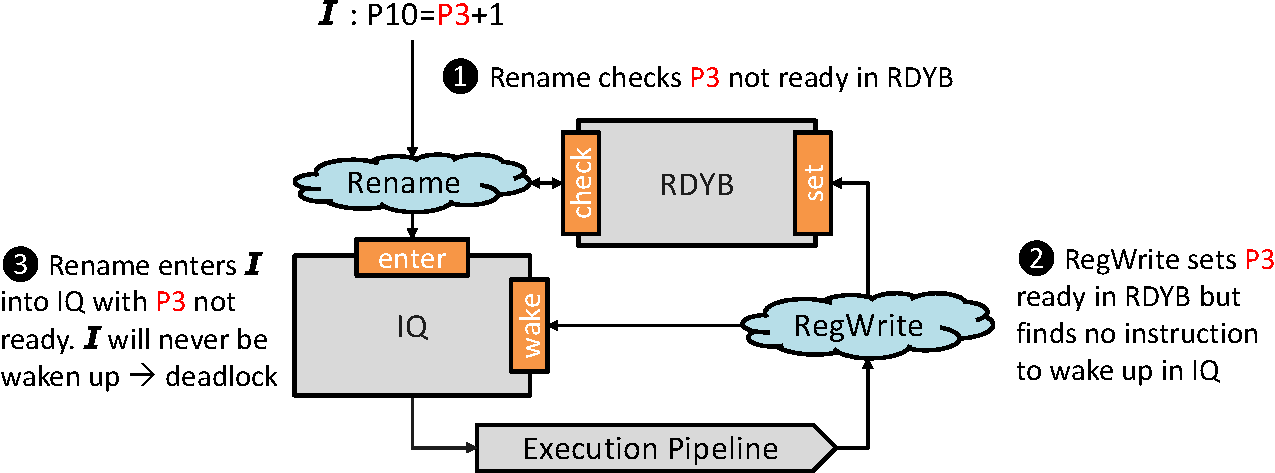
\includegraphics[width=\columnwidth]{figs/deadlock_cropped.pdf}}
    \caption{Race between microarchitectural events Rename and RegWrite in an OOO processor}\label{fig:race}
\end{figure}

\subsection{Maintaining Atomicity in CMD}
To resolve the race problem in Figure~\ref{fig:race}, CMD expresses events Rename and RegWrite as two separate rules and guarantees the atomicity of each rule.
That is, event Rename will be expressed as rule Rename which calls method \emph{check} of RDYB and method \emph{enter} of IQ, and event RegWrite will be expressed as rule RegWrite which calls method \emph{set} of RDYB and method \emph{wake} of IQ.
However, enforcing atomicity is challenging because the two rules manipulate the same states.
In this case, it has to be ensured that the rules appear to execute one after another.
Whether two rules can execute concurrently and in which order depend on the properties of the called methods.
Thus, for each module, we use a \emph{Conflict Matrix (CM)}, which specifies which methods of the module can be called concurrently.
The relation between each pair of methods may be described as follows:
\begin{itemize}
    \item \emph{conflict-free}: the methods do not manipulate the same state elements, and thus, can be called concurrently;
    \item \emph{conflicting}: the methods cannot be called in the same cycle;
    \item \emph{happen-before}: the methods can be called concurrently but functionally behave as if one executed before the other.
    This involves bypass logic inside the module in case a write method happens before a read method.
\end{itemize}
Given the CMs of all the modules, it is straightforward to derive the concurrency relation between every pair of rules.
Support for CMD requires a stall signal in the glue logic to suppress the execution of one rule in a pair of conflicting rules.

Back to the race problem in Figure~\ref{fig:race}, if there is no bypass wire in the implementation of module IQ or module RDYB, then the CM of IQ will have method \emph{wake} happen before \emph{enter}, and the CM of RDYB will have metho \emph{check} happen before \emph{set}.
In this case, rules Rename and RegWrite are conflicting with each other, and a stall signal will be generated by CMD to ensure atomicity.
To make rules RegWrite and Rename execute concurrently, one solution is to change the CM of RDYB to have method \emph{set} happen before \emph{check}.
This is, the implementation of module RDYB contains a bypass wire from method \emph{set} to \emph{check}.
We will show shortly that this bypass wire can be generated implicitly in CMD.
In this case, RegWrite will appear to execute before Rename.

\subsection{Expressing CMD in Hardware Description Languages (HDLs)}
We expressed the CMD framework in Bluespec System Verilog (BSV).
The BSV compiler automatically (1) derives the CM for each module implementation, (2) derives the concurrency relations between each pair of rules according to the CMs, and (3) generates stall signals in the glue logic.
\emph{The compiler statically resolves all the dynamic concurrency issues, making it possible to apply mechanical verification  techniques to designs.}

It is possible to use other HDLs to express CMD, but then we may not get all the benefits of the automatic concurrency analysis done by the BSV compiler.

\subsection{CMD Design Flow}
We develop designs in two phases.
We first focus on functionality and do not try to get maximum hardware concurrency.
After this phase, we often discover that two rules are conflicting, and this affects the performance adversely.
To execute such rules concurrently invariably requires introduction of bypass logic.
In CMD, one never writes bypass logic explicitly.
Instead, one can specify the order in which rules should execute, from which one can derive the desired CM of each module.
Rosenband~\cite{rosenband2004ephemeral} has given a systematic way to transform the module implementation to satisfy a given CM using Ephemeral History Registers (EHRs) which implicitly introduce bypass logic.
This transformation does not affect the functional correctness of the overall design.

\subsection{Modular Refinement in CMD}
When a refinement on a module does not affect the interface methods or the CM, the local correctness of the module guarantees the preservation of the overall correctness.
If the CM of the refined module is changed, the BSV compiler can re-analyze the relations between rules and generate stall new signals to keep the design functionally correct.

In some cases, a refinement may entail several modules simultaneously or may add new methods to a module for increased functionality.
Any changes in interface methods imply that the rules that call these methods have to be changed.
However, making this change does not require knowing the internal details of other modules, because other modules have been encapsulated by their interface specifications.

In summary, by employing modules with guarded interfaces and atomic rules, CMD is able to provide strong composability and atomicity.


\section{RiscyOO -- a RISC-V Out-of-Order Processor Designed Using CMD}\label{sec:ooo}
Using the CMD framework, we built, \emph{RiscyOO}, a parameterized out-of-order superscalar cache-coherent multiprocessor.
The processor uses the open-source RISC-V instruction set~\cite{riscv}.
Figure~\ref{fig:ooo} shows the structure of RiscyOO multiprocessor.
The OOO core contains 2-way superscalar fetch/decode/commit, 4 execution pipelines (only two are shown for simplicity), and two-level private TLBs.
The core also performs various branch predictions, and execute loads speculatively.
Multiple cores are connected to a non-blocking coherent cache hierarchy to form a multiprocessor.

\begin{figure}[!htb]
    \centering
    \subfloat[Top-level moduels and rules of the OOO core. Modules are represented by rectangles, while rules are represented  by clouds. The core contains four execution pipelines: two for ALU and branch instruction, one for memory instructions, and one for floating point and complex integer instructions (e.g. multiplication). Only two pipelines are shown here for simplicity.\label{fig:ooo:core}]{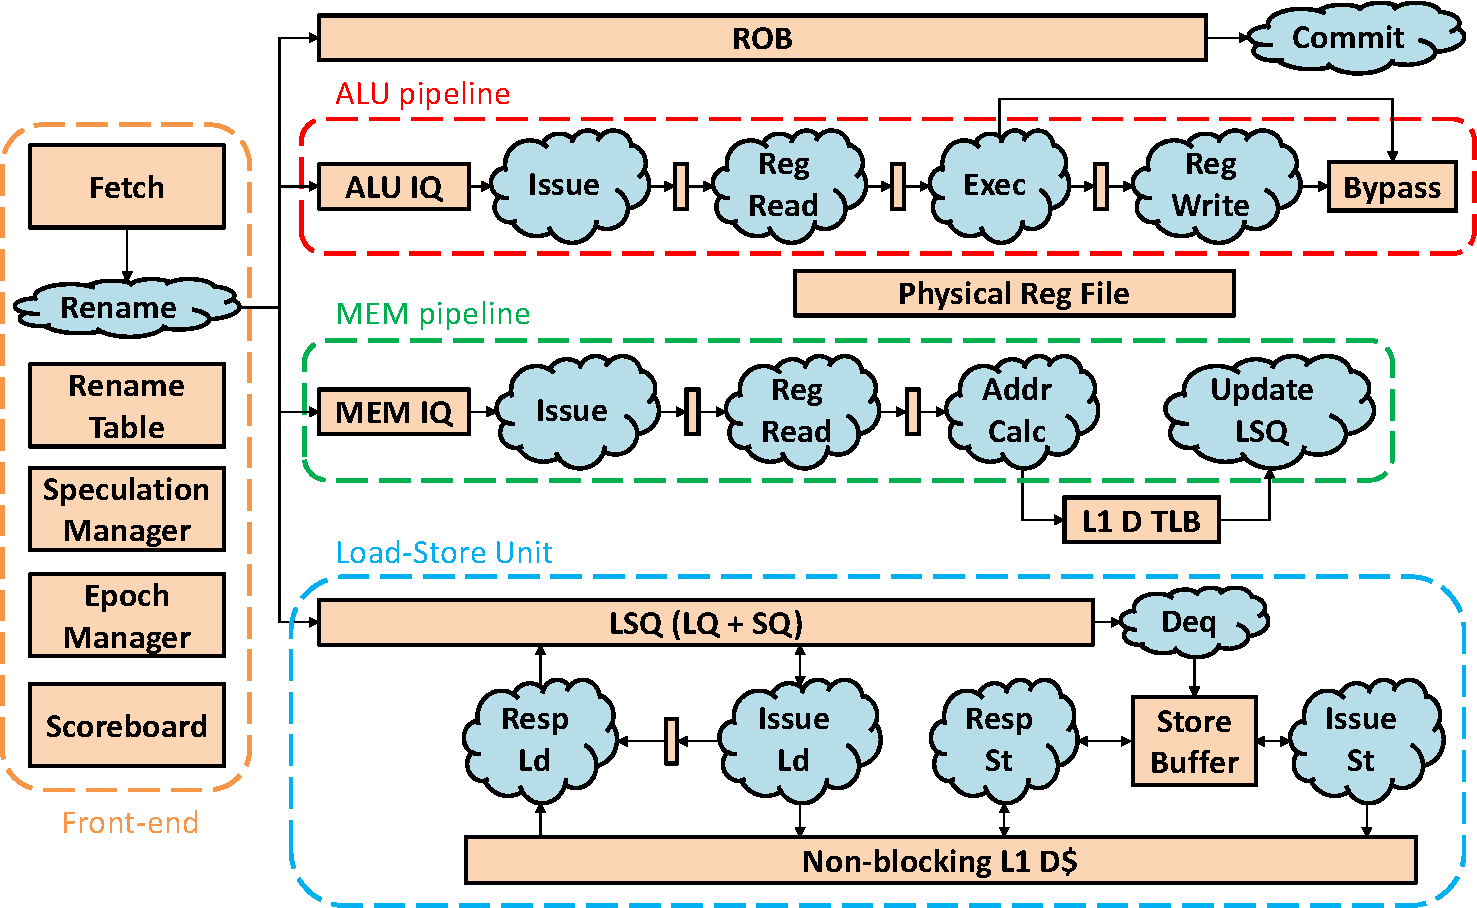
\includegraphics[width=\columnwidth]{figs/core_cropped.pdf}}\\
    \subfloat[Connecting OOO cores to form a multiprocessor\label{fig:ooo:mem}]{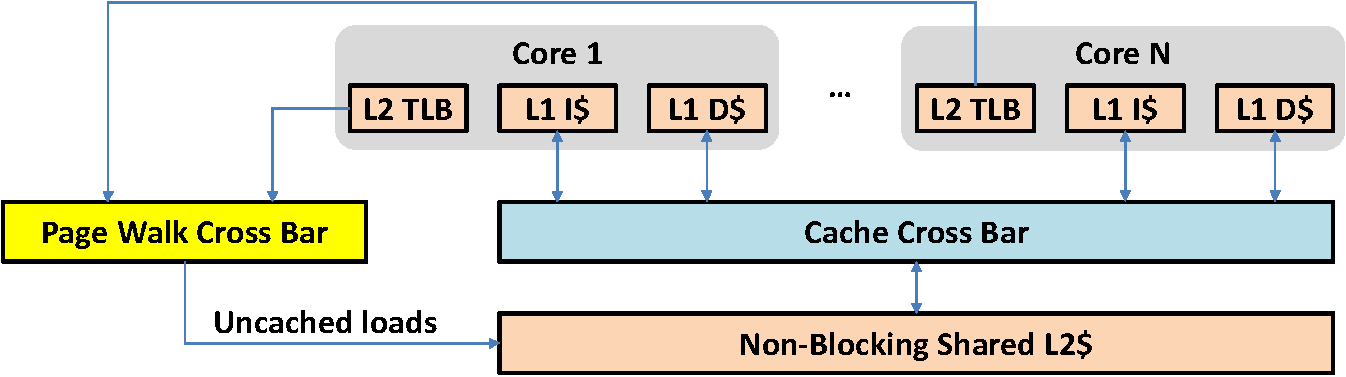
\includegraphics[width=0.9\columnwidth]{figs/mem_cropped.pdf}}
    \caption{RiscyOO multiprocessor}\label{fig:ooo}
\end{figure}

We prototyped RiscyOO on AWS F1 FPGA, and booted Linux on it.
To evaluate the performance of RiscyOO, we run SPEC CINT2006 benchmarks (ref input size, no sampling) which ran trillions of instructions on our FPGA prototype without any hardware failures.
Our evaluation shows that RiscyOO is much faster than in-order processors, and matches state-of-the-art academic out-of-order processors.
However, commercial ARM-based processors are 40\% faster than RiscyOO on average in terms of cycle counts, possibly because of the higher superscalarity and more sophisticated microarchitectures.
Detailed performance analysis can be found in \cite{riscyoo}.

We also applied standard ASIC synthesis flow (topographical synthesis) on RiscyOO.
Using a 32nm technology, the processor can be clocked over 1GHz.


\section{Applications of CMD and RiscyOO}\label{sec:app}

\subsection{Flexible Open-Source Processor IP}
The software community has benefited for years from open-source projects and permissive licensing. 
This has allowed reusable libraries with proper APIs to flourish. 
The open-source RISC-V ISA~\cite{riscv} is an attempt to open up the processor design community in a similar way.
Although there are already several good and free implementations of RISC-V processors~\cite{rocketchip,boom,pulp}, which can be included directly as processor IP blocks when building an SoC, they are not enough to realize the full potential of RISC-V.
This is because these processors are built in a structural way.
As a consequence, their customizability is at a coarse granularity (e.g., changing cache and buffer sizes) and often limited by the number of configurations provided by the original processor designers.
Moreover, if one needs to change the implementations of one or more modules in the processor, then he/she may need to understand the implementations of nearly all the modules in order to prevent his/her changes from breaking the whole processor.
This requires significant effort, which may be comparable to building a new processor from scratch, and we think it would intimidate people from reusing or customizing these processor IPs.

The CMD framework solves the problem by providing composability at the module level, and thus enables customization at a much finer granularity.
If people need to change a module in a processor designed using CMD, only the interfaces, instead of implementations, of other modules need to be understood.
This lowers the barrier for customizing processor designs, and would encourage more people to join the open-source hardware community.
Furthermore, CMD allows people to contribute a variety of modules and replacements, which can be composed easily using atomic rules to form processors suitable for different use cases.
As an example, we have made two refinements on RiscyOO, which we explain next.

\noindent\textbf{Refining the TLB microarhictectures:}
In the original design of RiscyOO, both L1 and L2 TLBs block on misses, and a L1 D TLB miss blocks the memory execution pipeline.
To improve performance, we have changed the L1 D TLB and L2 TLB to support parallel miss handling and hit-under-miss.
To reduce the TLB miss latency, we also included in the L2 TLB a split translation cache~\cite{translationCache}, which caches intermediate page walk results.
These refinements not only change the internal implementations of TLBs significantly, but also affect the interfaces of TLBs, e.g., the L1 D TLB sends responses out of order.
Thanks to CMD, the changes in TLBs affect only rules that call the TLB interfaces (e.g., rules AddrCalc and UpdateLSQ in Figure~\ref{fig:ooo:core}), and we were able to commit these changes within two weeks by one person.
Our evaluation shows that the refinements on TLBs can improve performance by 29\% on average~\cite{riscyoo}.

\noindent\textbf{Adding support for TSO:}
The original design of RiscyOO supported only a weak memory model WMM~\cite{wmm}.
To make RiscyOO support TSO, we have changed the design of the load-store unit and L1 D cache so that cache evictions from L1 D will be snooped by the load-store queue (LSQ in Figure~\ref{fig:ooo:core}).
These changes requires adding new interface methods, e.g., a new method in LSQ that kills eagerly executed loads when a cache eviction happens.
This new method can race with other existing methods in LSQ, e.g., the one that issues a load from LSQ.
Thanks to CMD, we can resolve these race conditions easily by relying on conflict matrices and rule-atomicity.
The TSO support was added by one person in two weeks.
We have run PARSEC benchmarks on a 4-core configuration of RiscyOO, and showed that the TSO refinement has little performance impact~\cite{riscyoo}.

To foster the open-source community, we have released our building blocks for the RiscyOO processor at \texttt{\url{https://github.com/csail-csg/riscy-OOO}} under the MIT License.
As the number of refinements on our design provided by us and the community grows over time, we hope these building blocks can become a toolbox for computer architects and SoC designers.

\subsection{Secure Architectures}
The recent advent of side-channel attacks based on speculative microarchitectures have prompted architects to redesign processors for security.
Such redesigns often manipulate microarchitectural states differently, and inevitably require changes in both software and hardware.
The RiscyOO processor is a great platform for exploring security solutions because its speculative microarchitecture is as vulnerable to side-channel attacks as commercial processors.
Its easy-to-modify modify design allows fast exploration of new security schemes which can be tested while running full software stack.
Since all the reported attacks can be replicated even in an FPGA implementation, a red team can directly try to break a supposedly ``secure'' processor running in the (AWS) cloud. 


\subsection{Substrate for Validating Software-Hardware Codesign}
\begin{comment}
When improving the PPA of processors, hardware changes that are transparent to software are most welcome, and if the benefits are high enough, they can be absorbed into commercial designs gradually.
However, with the end of Moore's law, hardware designs are facing more and more critical constraints, and it has become very difficult to come up with such transparent hardware changes to improve PPA.
\end{comment}
As many recent research proposals show, increasingly people have come to appreciate the importance of codesigning software and hardware.
However, these software-hardware codesign proposals meet with skepticism because of concerns about the interaction of architectural changes with the OS and other existing software/hardware stacks.
For example, proposals on adaptive cache architectures~\cite{Jigsaw} often need to color pages, and it is natural to be concerned about the changes in OS codes that are needed to do this correctly, or how the changes interact with super pages which can benefit applications with large memory footprints.
For another example, consider some newly proposed coherence protocols~\cite{DeNoVo}, which rely on software to be data-race-free (DRF). It is natural to have concerns regarding how the OS can gracefully terminate a user program that has data races and clean up polluted cache states caused by the user program.

It is almost impossible to address these system-level concerns using a simulator which does not run an OS.
Even if the simulator does run an OS, it is still difficult to convince others (e.g., commercial processor vendors) that the simulation model does not include anything that is difficult to implement in hardware.
More importantly, simulation models may omit details to gain simulation speed, but those omitted details may turn out to affect the proposed scheme.
For example, the DeNovo coherence protocol~\cite{DeNoVo}, which assumes software to be DRF, self-invalidates local caches at the end of each critical section.
To improve performance, it does not flush data read during the current critical section, because DRF software should always read up-to-date values.
However, the speculative load execution in modern processors may bring in any stale data into the local caches even when software is DRF.
The paper did not address this concern, because the evaluation was done using an one-IPC core model which did not even simulate wrong path instructions.

Given all the above concerns with software simulators, the only way to increase the fidelity of a software-hardware codesign proposal is to put up a full-system prototype.
Our RiscyOO processor would be a great substrate for building such prototypes.
Since RiscyOO boots Linux, researchers now have the opportunity to truly modify the OS and test the feasibility of the changes.
Furthermore, the CMD framework used to build RiscyOO allows researchers to implement the proposed changes in a short time.
In addition, the realistic microarchitectures of RiscyOO can help eliminate concerns on whether they have omitted hardware features that may affect the proposal adversely.
Last but not the least, the high speed of RiscyOO (40MHz on AWS F1 FPGA) makes evaluation of large realistic benchmarks possible.


\section{Conclusion}\label{sec:conclude}
To fully benefit from the openness of RISC-V, the architecture community needs a framework where many different people can cooperate to try out new ideas in real hardware.
Although existing chip generators can connect parameterized building blocks together,  they do not allow frequent changes to the building blocks.
We have also shown that latency-insensitive interfaces alone are insufficient in processor designs.
In this paper, we have proposed the CMD framework in which modules have guarded interface methods, and are composed together using atomic actions. 
With the atomicity guarantee in CMD, modules can be refined selectively relying only on the interface details, including Conflict Matrix, of other modules.
We have shown the efficacy of CMD by designing an OOO processor which has fairly complex architectural features.
Both the synthesis results and the performance results are very encouraging, and with sufficient effort by the community, it should be possible to deliver commercial grade OOO processors in not too distant a future.


\section*{Acknowledgment}
We thank all the anonymous reviewers for their helpful feedbacks on improving this paper.
We have also benefited from the help from Jamey Hicks and Muralidaran Vijayaraghavan.
We would like to particularly thank Bluespec, Inc. for providing free tool licenses.
This research is supported by the Defense Advanced Research Projects Agency (DARPA) under Contract No. FA8750-16-2-0004 (program BRASS) and Contract No. HR001118C0018 (program SSITH).
Any opinions, findings and conclusions or recommendations expressed in this material are those of the authors and do not necessarily reflect the views of the Defense Advanced Research Projects Agency (DARPA).


\bibliographystyle{IEEEtran}
\bibliography{top_picks}

\end{document}
